\subsubsection{Component Outcomes}
\label{sec:controlled-ablation}
\begin{table*}[t]\centering\scriptsize
\caption{Controlled amplitude-score and physical-state-carry ablation. Same five-model bank and publication rules. All 18 continuous parents (108 events) are retained. Normal controls comprise three 600-s records with 588 s evaluated exposure each (1,764 s total; startup excluded). Delay is conditional on emitted matched diagnoses and must be read with the no-timely-diagnosis count.}
\label{tab:a01}
\begin{tabular}{lrrrrrr}\toprule
Procedure & Timely & Extras & Normal FA & False restorations & No timely & Delay (s)\\\midrule
Marginal + carry & 108/108 & 1 & 0/1,764 s & 1 & 0/108 & 0.267\\
Profile + carry & 108/108 & 1 & 0/1,764 s & 1 & 0/108 & 0.267\\
Marginal + reset & 75/108 & 166 & 0/1,764 s & 130 & 33/108 & 0.337\\
Profile + reset & 75/108 & 166 & 0/1,764 s & 130 & 33/108 & 0.337\\
\bottomrule\end{tabular}\end{table*}

\begin{figure*}[t]\centering
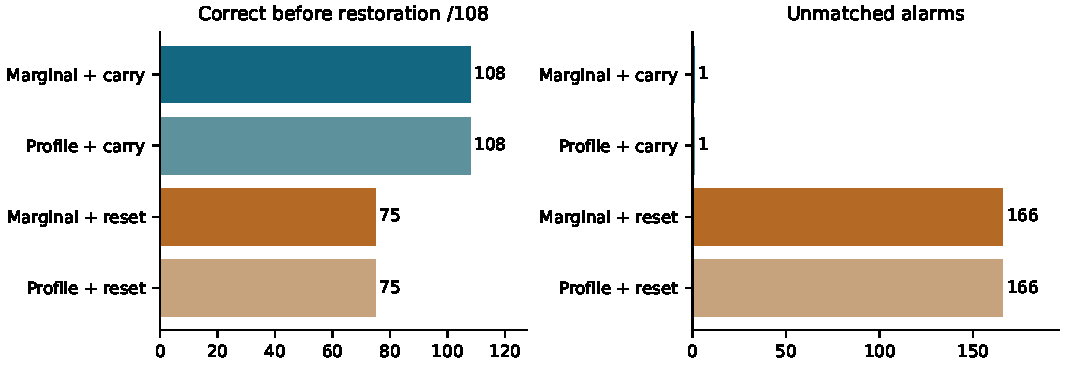
\includegraphics[width=.92\textwidth]{figures/generated/ablation_a01.pdf}
\caption{Amplitude-scoring and physical-state-carry ablation on identical
observations and five-model banks. The 108 interventions belong to 18
continuous trajectories. Thresholds are fixed, so the observed alarm rate
may differ between arms.}\label{fig:a01}\end{figure*}
Table~\ref{tab:a01} and Fig.~\ref{fig:a01} report coverage and alarm cost
for the four arms. With carry retained, marginal and bounded-profile
amplitude scores tie on the reported endpoints. Resetting the first 114
estimated physical-state deviations at inferred closure reduces timely
attribution and increases extras under both scores. This reset leaves
instrumental state, covariance regime, prior weights, thresholds, clocks
and reporting rules intact; simulated states and observations never reset.
The profile arm remains a normalized penalized score system and retains
conditional Bayesian state estimation. Thus this study supports a
physical-state-carry effect at inferred closure in the tested cohort, not
the necessity of Bayes or of every form of temporal memory. The supplement
reports denominators, normal exposure, persistent episodes, censoring and
all paired parent-cluster intervals. These are posthoc within-simulator
contrasts at the original thresholds, not a comparison at matched
false-alarm rates.
